\begin{figure}[bth!]
	\begin{center}
		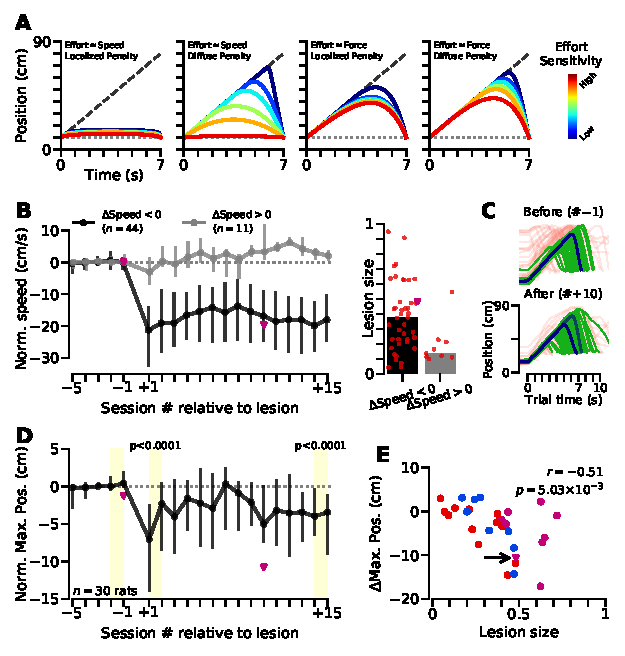
\includegraphics[scale=1]{ch-lesion/figures/MaxPosAnalysis.pdf}
		\caption
		{\textbf{Optimal trajectory vs effort sensibility and experimental validation.}
		\textbf{A)} Optimal trajectories predicted by models with different effort and spatial costs approximations.
		The cost of premature entrance in the reward area (spatial cost) was simulated using a Heaviside function that was either localized ($\sim$step function with non-zero value within the reward area) or diffuse ($\sim$a sigmoid function whose value gradually decreases toward zero away from the reward area).
		Effort was approximated as the square value of either the muscular force produced by the animals or of its speed.
		\textbf{B)} \textit{Left}, animals were divided into two groups based on the significance of the dS lesion effect on running speed.
		\textit{Right}, lesion size for animals in those two groups.
		\textbf{C)} Effect of striatal lesion on the trajectories of a single animal.
		Only trials in which the routine was executed (thin blue lines) were taken into account to compute the median trajectory (bold blue line).
		\textbf{D)} Effect of striatal lesion on the maximum position of the median trajectory across routine trials.
		\textbf{E)} Effect of striatal lesion on the maximum position versus lesion size.
		Same color code for individual lesion type as in \autoref{fig:lesion:task}.
		Green triangles in panels~B,~D, and~E are data points from the example animal whose trajectories, before and after lesion, are shown in panel~C.
		}
		\label{fig:lesion:maxPos}
	\end{center}
\end{figure}